\chapter{Heuristics for SQL Semantic Bug Detection}
\label{chapter:semantic_bugs_in_sql}

In this chapter we present in Section \ref{section:semantic_bugs} a detailed description of semantic bugs found in SQL queries as well as detection strategies for these in Section \ref{section:detection_strategies}. Furthermore, details about the implementation of the rule-based static analysis tool for detecting these bugs are given in Section \ref{section:implementation}. The process used for validating the tool is presented in Section \ref{section:validation} followed by the research methodology in Section \ref{section:research_methodology} and finally the results which are shown in Section \ref{section:results}.

\section{Semantic bugs in SQL queries}
\label{section:semantic_bugs}

A semantic bug in an SQL query, as defined by \citet{P001}, refers to a legal query which does not (always) produce the intended result. To be more precise, it means that the query uses correct SQL syntax, however the results it produces are incorrect for the given task, which means the query has some semantic bug. These are the types of errors that the tool presented in this paper tries to detect. This task is however non-trivial especially when there is no information about the task for which the query was written or how the queried data is structured. 

Semantic bugs are especially common to appear in queries written by students who are yet to master the SQL language, however these can also be present in real world applications, which makes them more dangerous. Since these issues do not usually generate any warnings from the database engines, it is therefore harder for inexperienced developers to catch them, especially due to the fact that in some cases the queries might actually seem to produce the correct results. For this very reason, it can be argued that semantic bugs in SQL are more dangerous than syntactic errors, which can very easily be detected as well as corrected. This is why tools for detecting these types of issues should be directly integrated in either development environments or even better, plugins that can check the correctness of queries during runtime.

Furthermore, semantic bugs can often impact the overall performance of the query leading to increased computation time or inefficient resource usage. This is again quite important in applications where speed is critical and executing queries which contain semantic bugs might lead to bottlenecks as discussed by \citet{P010} in their paper. Although previous studies did not show significant correlation between SQL code smells and other traditional code smells, it was shown by \citet{P010} that once an SQL semantic bug is introduced in some system, it tends to have a longer lifespan than other more traditional semantic code smells, which makes the task of detecting these types of errors quickly even more important.

\section{Detection strategies for SQL semantic bugs}
\label{section:detection_strategies}

In this section we propose several heuristics used for detecting semantic bugs in SQL queries. Each of these are later implemented as rules in the static analysis tool we developed for this project. The errors, which are detected by our proposed heuristics, were initially presented and classified in the work of \citet{P001} which represents a complete list of semantic bugs encountered in SQL. A small subset of semantic bugs was also collected from the SQL Enlight tool. This is a closed source static analysis tool developed by Yubitsoft Eood which aims to detect a number of issues in SQL queries as well. Other tools for SQL analysis and code smell detection are TOAD and SQL Prompt, both of which are also closed source and require a set of input queries as well as database schemas in order to detect any issues. Furthermore, none of the previously mentioned tools are able to analyse queries embedded in source code.

The rule-based static analysis tool developed for this project uses a hard implementation, meaning that the worst is always assumed, since there is no additional information related to tasks or database schemas. This means that for certain queries, the tool might generate false positive warnings, as will later be discussed in Section \ref{section:validation}, however this was preferred since it offers a good tradeoff for the setting when little information about the queries is known.

In the following subsections we provide a description of each bug, examples of SQL queries that contain the semantic bug and present the implementation of each detection strategy together with any assumptions made by the heuristics which are used in our tool. A summary of all the semantic bugs that our tool detects is also presented in Table \ref{table:semantic_issues}.

\begin{center}
\begingroup
\footnotesize
\begin{tabularx}{\linewidth}{XXXc}
\toprule
\textbf{Semantic bug} & \multicolumn{2}{X}{\textbf{Description}} & \textbf{Ref.} \\ \midrule
Inconsistent tuple variable                 & \multicolumn{2}{X}{Tuples matched on key attributes access different values for some other attribute}                                 & \cite{P001} \\ \hline
Constant output column                      & \multicolumn{2}{X}{The value of an output column is constant and can be derived from the query}                                       & \cite{P001} \\ \hline
Duplicate output column                     & \multicolumn{2}{X}{The same attribute is present inside the \sql{SELECT} clause multiple times}                                       & \cite{P001} \\ \hline
Unnecessary \sql{JOIN} clause               & \multicolumn{2}{X}{Tuple can be replaced with another already existing one (removing unnecessary join)}                               & \cite{P001} \\ \hline
Identical tuple variables                   & \multicolumn{2}{X}{Tuples matched on key attributes are identical}                                                                    & \cite{P001} \\ \hline
Comparison with \sql{NULL}                  & \multicolumn{2}{X}{Using normal comparison operators with \sql{NULL} instead of \sql{IS NULL} expression}                             & \cite{P001} \cite{P010} \\ \hline
Unnecessary general comparison              & \multicolumn{2}{X}{Using greater than or equals or less than or equals operators instead of the equals to operator}                   & \cite{P001} \\ \hline
\sql{LIKE} used without wildcards           & \multicolumn{2}{X}{Like can be replaced with equals to operator}                                                                      & \cite{P001} \cite{P995} \\ \hline
Unnecessary \sql{SELECT} list in \sql{EXISTS}    & \multicolumn{2}{X}{There is no need to add a complicated \sql{SELECT} list inside \sql{EXISTS} subqueries}                & \cite{P001} \\ \hline
Unnecessary index scan                      & \multicolumn{2}{X}{Using a wildcard character at the beginning of a string results in missing the access predicate}                   & \cite{P996} \\ \hline
Unnecessary \sql{DISTINCT} in aggregations  & \multicolumn{2}{X}{For certain aggregation function \sql{DISTINCT} keyword has no effect on the result}                               & \cite{P001} \cite{P997} \\ \hline
Unnecessary \sql{COUNT} argument            & \multicolumn{2}{X}{In certain cases the \sql{COUNT} argument is not necessary and can be replaced with something simple}              & \cite{P001} \\ \hline
Unnecessary \sql{GROUP BY} attribute        & \multicolumn{2}{X}{Attribute under \sql{GROUP BY} which does not appear under \sql{SELECT} or \sql{HAVING} outside aggregations is unnecessary}   & \cite{P001} \cite{P010} \\ \hline
Unnecessary \sql{GROUP BY} clause           & \multicolumn{2}{X}{If no aggregation functions are used, \sql{GROUP BY} can be replaced with \sql{SELECT DISTINCT}}                               & \cite{P001} \cite{P010} \\ \hline
Unnecessary \sql{UNION} condition           & \multicolumn{2}{X}{Two \sql{UNION} clauses with the same \sql{SELECT} and \sql{FROM} conditions and mutually exclusive \sql{WHERE} conditions can be merged}  & \cite{P001} \\ \hline
Unnecessary \sql{ORDER BY} terms            & \multicolumn{2}{X}{A constant term is not necessary to be included in the \sql{ORDER BY} clause}                                      & \cite{P001} \\ \hline
Unnecessary \sql{GROUP BY} terms            & \multicolumn{2}{X}{A constant term is not necessary to be included in the \sql{GROUP BY} clause}                                      & \cite{P001} \\ \hline
Inefficient \sql{HAVING} clause             & \multicolumn{2}{X}{Condition inside the \sql{HAVING} clause that can be moved inside the \sql{WHERE} clause making the query more efficient}      & \cite{P001} \\ \hline
Missing \sql{JOIN} conditions               & \multicolumn{2}{X}{Missing references for the joined tables}                                                                          & \cite{P001} \\ \hline
Uncorrelated \sql{EXISTS} subqueries        & \multicolumn{2}{X}{Subqueries contain no reference to tables or tuples defined in the higher level portions of the query}             & \cite{P001} \\ \hline
Mismatch in subquery \sql{SELECT}           & \multicolumn{2}{X}{For \sql{IN} subqueries, the \sql{SELECT} list from the inner query should match the attributes used in the outer query}      & \cite{P001} \\ \hline
Strange subquery conditions                 & \multicolumn{2}{X}{A condition inside an SQL subquery which accesses only tuple variables from the outer query is strange}            & \cite{P001} \\ \hline
Strange \sql{HAVING} clause                 & \multicolumn{2}{X}{A query using a \sql{HAVING} clause without a \sql{GROUP BY} clause is strange}                                    & \cite{P001} \\ \hline
Strange wildcards without \sql{LIKE}        & \multicolumn{2}{X}{Using wildcard characters without \sql{LIKE} is strange}                                                           & \cite{P001} \\ \hline
Division by zero                            & \multicolumn{2}{X}{Potential divisions by zero due to order of operation execution}                                                   & \cite{P001} \\ \hline
\caption{Summary of semantic bugs detected by our tool}
\label{table:semantic_issues}
\end{tabularx}
\endgroup
\end{center}

\subsection{Inconsistent tuple variable}
\emph{Motivation}: This bug is present whenever the key attributes of two different tuple variables over the same relation are matched while at the same time for some other attribute the two tuple variables are matched to different values. Since our tool does not require information about the database schema, we can not determine the key attributes, therefore the condition for this semantic bug is relaxed by dropping this constraint. More specifically, whenever two different tuple variables over the same relation have a set of attributes on which they are matched as well as at least one attribute for which there are different requirements, then this means the query is inconsistent, since the conditions can not be satisfied at the same time, hence the result set will be empty. The following example should be detected as having a semantic bug\footnote{\url{https://stackoverflow.com/questions/34064071/how-to-select-data-based-on-special-condition}}.

\begin{center}
\begin{tabular}{c}
\begin{lstlisting}[language=SQL]
SELECT * FROM audit a1 
WHERE NOT EXISTS (
SELECT * FROM audit a2 
WHERE a2.status='approve' AND a1.status='decline' AND a2.id=a1.id);
\end{lstlisting}
\end{tabular}
\end{center}

In this example, the two tuple variables \sql{a1} and \sql{a2} over the same relation \sql{audit} are being matched inside the \sql{EXISTS} subquery on the \sql{id} attribute, however, the query is inconsistent since \sql{a1.status = 'decline'} and \sql{a2.status = 'approve'} can not have two different values at the same time, hence the result set for this subquery will always be empty. A potential fix for the example query is given below.

\begin{center}
\begin{tabular}{c}
\begin{lstlisting}[language=SQL]
SELECT * FROM audit a1;
\end{lstlisting}
\end{tabular}
\end{center}

\noindent \emph{Detection strategy}: Detecting this semantic bug is done by building, for each tuple variable used, a set of attributes which are equated with other tuple variables over the same relation. Furthermore, a second set is built which stores the attributes that are equated with other constant values. After the query is parsed, for all tuple variables over the same relation, we check the set of matching attributes as well as the set of attributes which are equated to different values. If there is a full match between the attributes in the first set, then we check to see whether there are any common attributes from the second set which might be equated to different values. If this is the case, then the query has inconsistent conditions and a warning for this semantic bug is generated by our tool.

\subsection{Constant output column}
\emph{Motivation}: This semantic bug appears whenever the value of an output column is constant and can be derived from the query without any additional information regarding the state of the database. More specifically, whenever an attribute under the \sql{WHERE} clause is equated to some constant value, if it is also present in the \sql{SELECT} list, then it will always have the same value. This attribute can therefore be removed from the \sql{SELECT} clause. The following example should be detected as having a semantic bug\footnote{\url{https://stackoverflow.com/questions/16449377/combine-two-queries-to-check-for-duplicates-in-mysql}}.

\begin{center}
\begin{tabular}{c}
\begin{lstlisting}[language=SQL]
SELECT * FROM person WHERE name = 'robert';
\end{lstlisting}
\end{tabular}
\end{center}

In this example, there is a constant column which is present in the output of the query, more specifically the \sql{name} attribute is equated to some constant value, thus it can be removed from the \sql{SELECT} clause. We can not directly provide a potential fix for this query without having more information about the structure of the \sql{person} schema, however the query can easily be corrected by specifying only the individual columns that are needed.\\

\noindent \emph{Detection strategy}: This bug is detected by looking for attributes under the \sql{WHERE} clause which are equated to some constant value. If this attribute is also present under the \sql{SELECT} clause or the select all operator (\sql{*}) is used, then it means that it will always have a constant value, hence it can be removed from the output, and a warning indicating this will be generated by our tool.

\subsection{Duplicate output column}
\emph{Motivation}: This bug appears when the \sql{SELECT} list of a query or subquery contains the same attribute multiple times. In this case, it means that duplicate output columns will be present in the result set, therefore these columns can be removed from the \sql{SELECT} clause, making the query easier to understand. The following example should be detected as having a semantic bug\footnote{\url{https://stackoverflow.com/questions/10845201/tsql-join-query}}.

\begin{center}
\begin{tabular}{c}
\begin{lstlisting}[language=SQL]
SELECT e.empid, e.fname, c.description AS hair, c.description AS race 
FROM employee2 e INNER JOIN code c;
\end{lstlisting}
\end{tabular}
\end{center}

In this example, there is a duplicate output column, since the \sql{c.description} attribute is specified two times under the \sql{SELECT} clause of the query. A potential fix for the example query is given below.

\begin{center}
\begin{tabular}{c}
\begin{lstlisting}[language=SQL]
SELECT e.empid, e.fname, c.description AS hair_or_race 
FROM employee2 e INNER JOIN code c;
\end{lstlisting}
\end{tabular}
\end{center}

\noindent \emph{Detection strategy}: For detecting this semantic bug, the \sql{SELECT} clause as well as the \sql{FROM} clause of each query is parsed. We then keep track of tuple variables declared in the \sql{FROM} clause and referenced under \sql{SELECT}, in order to detect different tuple variables referring to the same attribute. All attributes present in the \sql{SELECT} clause are then verified in order to determine whether there are duplicates in this list. Furthermore, if the select all operator (\sql{*}) is present, then there is also no need for selecting other attributes.

\subsection{Unnecessary \sql{JOIN} clause}
\emph{Motivation}: This bug appears in queries containing a tuple variable \sql{A}, for which only the key attributes are accessed, and this key is then equated with the foreign key of another tuple variable \sql{B}. In this case, the tuple variable A is not needed, as this results in an unnecessary \sql{JOIN} being used. This semantic bug can therefore have an impact on the performance of the query and should be corrected. For our tool, the requirement on key attributes is dropped, since only the query is presented as input, and there is no way of detecting which attributes represent the keys for a tuple variable. Therefore, we check if for some tuple variable \sql{A}, the attributes which are being accessed for it are then further equated with the same attributes of another tuple variable \sql{B}, in which case \sql{A} might not be needed, resulting in the unnecessary \sql{JOIN}. The following example should be detected as having a semantic bug\footnote{\url{https://stackoverflow.com/questions/25953303/multiple-select-result-in-mysql-depend-on-other-select}}.

\begin{center}
\begin{tabular}{c}
\begin{lstlisting}[language=SQL]
SELECT t.* FROM terms t 
JOIN term_relationships tr ON tr.term_id = t.term_id 
JOIN posts p ON p.post_id = tr.post_id WHERE p.post_id = 1;
\end{lstlisting}
\end{tabular}
\end{center}

In this example, there is an unnecessary \sql{JOIN} for \sql{posts} on \sql{post_id} since the condition inside the \sql{WHERE} clause, \sql{p.post_id = 1}, can be replaced by \sql{tr.post_id = 1} and moved up inside the second \sql{JOIN} clause. This not only helps with making the query easier to understand, but also improves the performance of the query since there is one less \sql{JOIN} that needs to be executed. A potential fix for the example query is given below.

\begin{center}
\begin{tabular}{c}
\begin{lstlisting}[language=SQL]
SELECT t.* FROM terms t 
JOIN term_relationships tr ON tr.term_id = t.term_id 
WHERE tr.post_id = 1;
\end{lstlisting}
\end{tabular}
\end{center}

\noindent \emph{Detection strategy}: Detecting this semantic bug is done by keeping track, for each tuple variable, of the comparisons in which they are involved throughout the query. After the query is parsed, for each tuple variable \sql{A}, we check all the comparison expressions in which it was used. If all accessed attributes are also equated with a different tuple variable \sql{B}, under the assumption that these attributes are a foreign key of this tuple variable \sql{B}, then a warning for an unnecessary \sql{JOIN} is raised.

\subsection{Identical tuple variables}
\emph{Motivation}: If a query contains two different tuple variables over the same relation for which the key attributes are equated, then these two variables must always point to the same tuple. Since our tool does not take as input any information regarding the key attributes of the schema for which the query was written, the detection rule checks for tuple variables over the same relation for which at least one attribute is equated, with the assumption that this attribute represents the key. In some cases, this might not hold and the generated warning should then be considered as a false positive. The following example should be detected as having a semantic bug.

\begin{center}
\begin{tabular}{c}
\begin{lstlisting}[language=SQL]
SELECT * FROM employees X, employees Y WHERE X.employee_id=Y.employee_id;
\end{lstlisting}
\end{tabular}
\end{center}

In this example, the two tuple variables \sql{X} and \sql{Y} over the same relation \sql{employees} are matched on \sql{employee_id}, thus under the assumption that this is a unique key, the two tuple variables are identical, meaning they will always refer to the same rows. In this case, we can not directly provide a potential fix for this query without having more information about the structure of the \sql{employees} schema and the underlying task for which the query was written.\\

\noindent \emph{Detection strategy}: The implementation for detecting this semantic bug first stores all tuple variables used in the query as well as the tables to which the variables refer. Whenever the equals to operator is detected, we check to see whether the tuple variables used in the comparison are pointing to the same underlying table and the same attribute is used on both sides of the comparison. If this is the case, under the assumption that the compared attribute represents a unique key on the table, then the two tuple variables must always point to the same tuple, thus they are identical and a warning is generated indicating the presence of this semantic bug.

\subsection{Comparison with \sql{NULL}}
\emph{Motivation}: In some database management systems it is syntactically valid to use \sql{A = NULL}, however this expression always has a constant truth value of either null or unknown. To avoid such situations, the \sql{IS NULL} or \sql{IS NOT NULL} should always be used instead. The following example should be detected as having a semantic bug\footnote{\url{https://stackoverflow.com/questions/52203347/check-if-field-exists-in-cosmosdb-json-with-sql-nodejs}}.

\begin{center}
\begin{tabular}{c}
\begin{lstlisting}[language=SQL]
SELECT r.id, r.authtoken.instagram, r.username FROM root r 
WHERE r.abc <> null;
\end{lstlisting}
\end{tabular}
\end{center}

In this example, \sql{r.abc} is being compared to \sql{null}. For some database engines, this might not be considered a syntactic error, however the condition will return either null or unknown. To avoid these types of situations, when \sql{null} is involved, we should always use the \sql{IS NULL} or \sql{IS NOT NULL} expressions instead of the comparison operators. A potential fix for the example query is given below.

\begin{center}
\begin{tabular}{c}
\begin{lstlisting}[language=SQL]
SELECT r.id, r.authtoken.instagram, r.username FROM root r 
WHERE r.abc IS NOT null;
\end{lstlisting}
\end{tabular}
\end{center}

\noindent \emph{Detection strategy}: For detecting this semantic bug, whenever the equals to or not equals to operators are used inside a query, we check to see whether one of the terms is the \sql{NULL} keyword. If this is the case, then the comparison operator should be replaced with the expression \sql{IS NULL} or \sql{IS NOT NULL} respectively.

\subsection{Unnecessary general comparison}
\emph{Motivation}: This semantic bug concerns the greater than or equals as well as the less than or equals operators. When the greater than or equals operator is used inside the \sql{WHERE} clause and the rightmost term of the comparison operator contains a subquery where the \sql{SELECT} list only uses the \sql{MAX} function with the same attribute as the leftmost comparison term, then the greater than or equals can be replaced with the equals operator. Similarly, the same holds for the less than or equals operator and the \sql{MIN} function. The following example should be detected as having a semantic bug\footnote{\url{https://stackoverflow.com/questions/43248530/max-or-all-in-sql}}.

\begin{center}
\begin{tabular}{c}
\begin{lstlisting}[language=SQL]
SELECT name FROM world 
WHERE gdp >= (SELECT max(gdp) FROM world WHERE continent = 'europe');
\end{lstlisting}
\end{tabular}
\end{center}

In this example, the greater than or equals operator from within the \sql{WHERE} clause can be replaced by the equals operator, because of the \sql{SELECT max(gdp)} expression from the subquery, which will make the query easier to understand. A potential fix for the example query is given below.

\begin{center}
\begin{tabular}{c}
\begin{lstlisting}[language=SQL]
SELECT name FROM world 
WHERE gdp = (SELECT max(gdp) FROM world WHERE continent = 'europe');
\end{lstlisting}
\end{tabular}
\end{center}

\noindent \emph{Detection strategy}: This semantic bug is detected by checking the greater than or equals or less than or equals operators inside the \sql{WHERE} clauses of queries. Whenever such operators are detected, the clause following the operator is checked in order to determine whether a \sql{SELECT MAX} or \sql{SELECT MIN} is used, where the \sql{MAX} and \sql{MIN} functions use the same attribute as the leftmost term of the comparison operator. In these cases, the comparison can be replaced by the equality operator making the query easier to understand.

\subsection{\sql{LIKE} used without wildcards}
\emph{Motivation}: If a query uses a \sql{LIKE} expression which does not contain any wildcard characters, then the \sql{LIKE} can and should be replaced by the equals to operator. When using the equality operator, the entire strings are compared as opposed to comparing one character at a time when the \sql{LIKE} expression is used without any wildcards. The following example should be detected as having a semantic bug\footnote{\url{https://stackoverflow.com/questions/6502134/query-for-exact-match-of-a-string-in-sql}}.

\begin{center}
\begin{tabular}{c}
\begin{lstlisting}[language=SQL]
SELECT description FROM tproduct WHERE description LIKE 'diamond';
\end{lstlisting}
\end{tabular}
\end{center}

In this example, the \sql{LIKE} expression is used, however it does not contain any wildcard characters. In this case, the \sql{LIKE} expression can be replaced by the equality operator. A potential fix for the example query is given below.

\begin{center}
\begin{tabular}{c}
\begin{lstlisting}[language=SQL]
SELECT description FROM tproduct WHERE description = 'diamond';
\end{lstlisting}
\end{tabular}
\end{center}

\noindent \emph{Detection strategy}: For detecting this bug, the \sql{LIKE} expressions from within the parsed query are checked in order to see whether any wildcard characters are being used. If this is not the case, a warning is raised indicating the presence of this semantic bug.

\subsection{Unnecessary \sql{SELECT} list in \sql{EXISTS} clause}
\emph{Motivation}: When using an \sql{EXISTS} subquery, the \sql{SELECT} list from the subquery is not important since \sql{EXISTS} only checks for row existence, independent of the selected columns. When the query is executed, as soon as the \sql{EXISTS} subquery returns one row, its execution is stopped and \sql{TRUE} is returned to the parent query. Therefore, in \sql{EXISTS} subqueries, the \sql{SELECT} list is not important and something simple such as the select all operator (\sql{*}) should be used. However, this does not hold for \sql{IN} subqueries, where the \sql{SELECT} list from within the subquery is indeed important. The following example should be detected as having a semantic bug\footnote{\url{https://stackoverflow.com/questions/27633978/compare-combination-of-two-column-with-combination-of-other-two-in-sql}}.

\begin{center}
\begin{tabular}{c}
\begin{lstlisting}[language=SQL]
SELECT id, name FROM tbl_bkp t1 
WHERE NOT EXISTS (
SELECT id, name FROM tbl_namecode WHERE id=t1.id AND name = t1.name);
\end{lstlisting}
\end{tabular}
\end{center}

In this example, inside the \sql{EXISTS} subquery, the \sql{SELECT} list contains multiple attributes. This is redundant as the only \sql{TRUE} or \sql{FALSE} will be returned to the parent query, therefore the \sql{SELECT} list can be replaced with something simpler such as the select all operator. A potential fix for the example query is given below.

\begin{center}
\begin{tabular}{c}
\begin{lstlisting}[language=SQL]
SELECT id, name FROM tbl_bkp t1 
WHERE NOT EXISTS (
SELECT * FROM tbl_namecode WHERE id=t1.id AND name = t1.name);
\end{lstlisting}
\end{tabular}
\end{center}

\noindent \emph{Detection strategy}: Detecting this semantic bug is done by parsing the query and searching for \sql{EXISTS} subqueries. When these are detected, the \sql{SELECT} list is checked and if it does not use a simple operator such as the select all operator or a single attribute, then a warning for this bug is raised.

\subsection{Unnecessary index scan}
\emph{Motivation}: This semantic bug concerns the use of wildcard characters used at the beginning of a word while searching with the \sql{LIKE} operator. In SQL, the usage of the \sql{LIKE} operator is often the cause of unexpected performance issues because of inefficient indexing. The position of the wildcard characters inside the word that is being matched can cause significant drops in performance. When using a \sql{LIKE} filter, only the characters which appear before the first wildcard can be used as indices to speed up the pattern matching. The remaining characters are just filter predicates which do not help with reducing the scanned index range. Therefore, \sql{LIKE} expressions can contain an access predicate, the part before the first wildcard, and the filter predicate, the remaining characters. The scanned index range becomes smaller if the access predicate is more selective, resulting in better performance for the queries since the index lookup is faster. Thus, if a \sql{LIKE} expression starts with a wildcard character, then no access predicate is present which defeats the purpose of an index, resulting in a scan of the entire database table. The following example should be detected as having a semantic bug\footnote{\url{https://stackoverflow.com/questions/11754192/like-operator-to-retrieve-the-results}}.

\begin{center}
\begin{tabular}{c}
\begin{lstlisting}[language=SQL]
SELECT * FROM street WHERE street_name LIKE '%park%ave%10%';
\end{lstlisting}
\end{tabular}
\end{center}

In this example, the search term for the \sql{LIKE} expression starts with a wildcard character (matching zero or more characters), therefore there is no access predicate, thus the query will perform a full table index scan. In order to optimize the query it would be better to either provide an access predicate or, in case this is not possible, use a search function which will result in a full text index scan. In this case, the query can be fixed by using the \sql{MATCH} and \sql{AGAINST} syntax. The \sql{MATCH} operator takes as input a comma separated list which names the columns to be searched, while the \sql{AGAINST} clause takes as input the string to search for together with an optional modifier that includes the type of search. This can either be a natural language search, a boolean search or a query expansion search. A potential fix for the example query is given below.

\begin{center}
\begin{tabular}{c}
\begin{lstlisting}[language=SQL]
SELECT * FROM street WHERE MATCH(street_name) 
AGAINST('park ave 10' WITH QUERY EXPANSION);
\end{lstlisting}
\end{tabular}
\end{center}

\noindent \emph{Detection strategy}: The implementation for detecting this semantic bug parses the query in search for \sql{LIKE} expressions. Whenever such an expression is found, the search term is checked in order to determine whether or not it starts with a wildcard character. If this is the case, a warning is generated indicating that an access predicate is missing, thus a full index scan will be performed.

\subsection{Unnecessary \sql{DISTINCT} in aggregations}
\emph{Motivation}: For the \sql{MIN} and \sql{MAX} aggregation functions the \sql{DISTINCT} keyword is never necessary since this has no effect on the underlying query results. Furthermore, in most cases the presence of duplicates is likely significant in computing the results of the \sql{SUM} and \sql{AVG} aggregation functions, thus duplicates should not be excluded unless there are strong reasons for this. Therefore, the presence of the \sql{DISTINCT} keyword inside these aggregation functions is strange and should raise a warning. For the other aggregation functions, it can not be determined whether \sql{DISTINCT} is necessary or not inside the clause without having additional information about the query task, thus the other aggregation functions are excluded from this check. The following example should be detected as having a semantic bug\footnote{\url{https://stackoverflow.com/questions/53067977/combine-two-tables-unique-column}}.

\begin{center}
\begin{tabular}{c}
\begin{lstlisting}[language=SQL]
SELECT SUM(DISTINCT money) AS sum_money, m.created_at FROM receipt r 
JOIN material m GROUP BY m.created_at;
\end{lstlisting}
\end{tabular}
\end{center}

In this example, the \sql{DISTINCT} keyword is used inside the \sql{SUM} function. Unless there are strong reasons for this, the presence of \sql{DISTINCT} here is considered strange since duplicates are most likely significant in this case, however without having additional information about the task for which the query was written, our tool will raise a warning for a potential semantic bug. Without having more information about the underlying task for which the query was written, we can not provide a potential fix for this query.\\

\noindent \emph{Detection strategy}: The detection strategy checks whether any of the \sql{MIN}, \sql{MAX}, \sql{SUM} or \sql{AVG} aggregation functions are present in the query. For each of them, it then detects whether the \sql{DISTINCT} keyword was used inside the function clause and if so a warning is raised.

\subsection{Unnecessary \sql{COUNT} argument}
\emph{Motivation}: The \sql{COUNT} aggregation function can be used with or without an argument, in which case the star symbol is used (\sql{*}) most commonly. Whenever there is no \sql{DISTINCT} being used in the \sql{COUNT} function and the argument can not be null, these two versions of the \sql{COUNT} function are equivalent and the one without any argument is preferred since it makes the query easier to understand and read. In our implementation for this detection strategy, we can not check the condition related to the arguments of the \sql{COUNT} function not being null, since this would require additional information about the database schemas, therefore we make the assumption that the arguments used inside the \sql{COUNT} functions are not null. The following example should be detected as having a semantic bug\footnote{\url{https://stackoverflow.com/questions/761700/how-can-i-check-for-average-concurrent-events-in-a-sql-table-based-on-the-date}}.

\begin{center}
\begin{tabular}{c}
\begin{lstlisting}[language=SQL]
SELECT m.time, COUNT(r.seconds) FROM dbo.minutes m GROUP BY m.time;
\end{lstlisting}
\end{tabular}
\end{center}

In this example, there is no \sql{DISTINCT} being used in the \sql{COUNT} function and only one argument is used. Therefore, the clause inside the \sql{COUNT} can be simplified and the start operator can be used instead. A potential fix for the example query is given below.

\begin{center}
\begin{tabular}{c}
\begin{lstlisting}[language=SQL]
SELECT m.time, COUNT(*) FROM dbo.minutes m GROUP BY m.time;
\end{lstlisting}
\end{tabular}
\end{center}

\noindent \emph{Detection strategy}: For detecting this semantic bug, we parse the query and check if any \sql{COUNT} functions are being used. For each of these, we then check whether \sql{DISTINCT} is used inside the \sql{COUNT} clause. If this is not the case, and the clause only contains an argument, then we raise a warning indicating that the \sql{COUNT} clause can be simplified by using the start operator instead.

\subsection{Unnecessary \sql{GROUP BY} attribute}
\emph{Motivation}: Whenever an attribute which appears under the \sql{GROUP BY} clause is functionally determined by other attributes and if it does not appear under the \sql{SELECT} or \sql{HAVING} clauses outside of aggregation functions, then it can be removed from the \sql{GROUP BY} altogether. For our tool, this condition is relaxed since we are looking only at the query without knowing the database schema, thus it can not be determined whether an attribute is functionally determined by other attributes or not. Therefore, we only check for an attribute which appears inside the \sql{GROUP BY} clause without being used in either the \sql{SELECT} or \sql{HAVING} clauses outside of any aggregation functions, in which case a warning for this semantic bug will be triggered. The following example should be detected as having a semantic bug\footnote{\url{https://stackoverflow.com/questions/4818207/sql-aggragates-and-aliass}}.

\begin{center}
\begin{tabular}{c}
\begin{lstlisting}[language=SQL]
SELECT count(*) AS countbyid FROM items 
WHERE fkid = 2003799 GROUP BY fkid 
HAVING countbyid>1 ORDER BY countbyid;
\end{lstlisting}
\end{tabular}
\end{center}

In this example, the \sql{fkid} attribute is present under the \sql{GROUP BY} clause without being used in either the \sql{SELECT} or the \sql{HAVING} clauses outside aggregation functions, therefore it can be removed from the \sql{GROUP BY}. This will further simplify the query since the \sql{fkid} is the only attribute present under \sql{GROUP BY}. Furthermore, this query contains another semantic bug since \sql{fkid} can only have one value as it is equated to some constant in the \sql{WHERE} clause, thus the grouping will have no effect on the result. A potential fix for the example query is given below.

\begin{center}
\begin{tabular}{c}
\begin{lstlisting}[language=SQL]
SELECT count(*) AS countbyid FROM items 
WHERE fkid = 2003799 
HAVING countbyid>1 ORDER BY countbyid;
\end{lstlisting}
\end{tabular}
\end{center}

\noindent \emph{Detection strategy}: The detection strategy for this bug parses the query and keeps track of the attributes appearing under the \sql{SELECT} and \sql{HAVING} clauses outside of aggregation functions. Furthermore, the attributes appearing under the \sql{GROUP BY} clause are also stored. When the parsing of the query is finished, we check for attributes found under the \sql{GROUP BY} clause that are not present in either of the two lists with attributes detected inside \sql{SELECT} or \sql{HAVING} clauses. For each of these attributes a warning is raised indicating this semantic bug being detected in the query.

\subsection{Unnecessary \sql{GROUP BY} clause}
\emph{Motivation}: If a query has exactly the same attributes under the \sql{SELECT} clause listed inside the \sql{GROUP BY} clause as well and if no aggregation functions are used in either of the two clauses, then the \sql{GROUP BY} clause can be replaced by \sql{SELECT DISTINCT}. In most cases, the SQL optimizer will produce the same or similar execution plans for the two queries, so in these cases there is not always a gain in terms of performance, however by rewriting the query this becomes shorter and clearer. In most of these cases, using the \sql{GROUP BY} clause essentially removes duplicates from the result set, therefore the \sql{DISTINCT} operator is better suited to be used, as opposed to situations where aggregation functions are used in which case a \sql{GROUP BY} is indeed required. The following example should be detected as having a semantic bug\footnote{\url{https://stackoverflow.com/questions/33840072/how-can-you-have-a-column-equal-all-items-in-a-list}}.

\begin{center}
\begin{tabular}{c}
\begin{lstlisting}[language=SQL]
SELECT p.name FROM pc p LEFT JOIN sc s ON p.color=s.color 
WHERE s.color IS NOT NULL GROUP BY p.name;
\end{lstlisting}
\end{tabular}
\end{center}

In this example, all the \sql{SELECT} attributes are listed under the \sql{GROUP BY} clause and also no aggregation functions are used, therefore the \sql{GROUP BY} clause can be dropped and replaced by \sql{SELECT DISTINCT}, making the query shorter and clearer. A potential fix for the example query is given below.

\begin{center}
\begin{tabular}{c}
\begin{lstlisting}[language=SQL]
SELECT DISTINCT p.name FROM pc p LEFT JOIN sc s ON p.color=s.color 
WHERE s.color IS NOT NULL;
\end{lstlisting}
\end{tabular}
\end{center}

\noindent \emph{Detection strategy}: The implementation for this strategy first checks whether any aggregation functions are used in either the \sql{SELECT} or the \sql{GROUP BY} clauses. If this is the case, then there is no need to continue with further checking the query for this semantic bug. Otherwise, we continue by detecting all the terms used in the \sql{SELECT} clause as well as those used under the \sql{GROUP BY} clause. If there is a perfect match between these two sets of terms, then it means that the \sql{GROUP BY} clause can be replaced by a \sql{SELECT DISTINCT} and a warning for this semantic bug is triggered.

\subsection{Unnecessary \sql{UNION} condition}
\emph{Motivation}: A query for which the two \sql{UNION} subqueries use the same \sql{SELECT} expressions, the same \sql{FROM} lists as well as mutually exclusive \sql{WHERE} conditions, can be simplified by joining the two \sql{WHERE} clauses and connecting them using an \sql{OR}, replacing the \sql{UNION} altogether. The same holds for queries using a \sql{UNION ALL} clause, in which case the query can again be simplified and the two different \sql{WHERE} clauses joined using an \sql{OR}. For our tool, the condition for mutually exclusive \sql{WHERE} conditions can not be fully checked without having additional database schema information, therefore this was relaxed to only having different \sql{WHERE} clause expressions. The following example should be detected as having a semantic bug\footnote{\url{https://stackoverflow.com/questions/4715820/how-to-order-by-with-union-in-sql}}.

\begin{center}
\begin{tabular}{c}
\begin{lstlisting}[language=SQL]
SELECT id, name, age FROM student WHERE age < 15 UNION 
SELECT id, name, age FROM student WHERE name LIKE '%a%' ORDER BY name;
\end{lstlisting}
\end{tabular}
\end{center}

In this example, the query contains one \sql{UNION} clause and we can observe that the \sql{SELECT} expressions of the two subqueries are the same as well as the \sql{FROM} lists, more specifically the same table \sql{student} is used in both subqueries. Furthermore, the two \sql{WHERE} clauses are mutually exclusive, therefore, the query can be simplified by replacing the \sql{UNION} with an \sql{OR} and joining the two \sql{WHERE} clauses. This query also suffers from another semantic bug, more specifically the unnecessary index scan, since the \sql{LIKE} expression is starting with a wildcard character. A potential fix for the example query is given below.

\begin{center}
\begin{tabular}{c}
\begin{lstlisting}[language=SQL]
SELECT id, name, age FROM student WHERE age < 15 OR 
MATCH(name) AGAINST ('a' WITH QUERY EXPANSION) 
ORDER BY name;
\end{lstlisting}
\end{tabular}
\end{center}

\noindent \emph{Detection strategy}: The implementation for this strategy first detects whether the query involves any \sql{UNION} or \sql{UNION ALL} clauses. If this is the case, then we continue  with storing the \sql{SELECT} expressions, as well as the \sql{FROM} lists and the expressions under the \sql{WHERE} clauses. After the whole query is parsed, we pairwise check the collected lists involving the three different clauses. Whenever two \sql{SELECT} list expressions as well as \sql{FROM} lists from two different subqueries are the same, the \sql{WHERE} clauses are checked and if different then a warning is triggered, informing the user that the \sql{UNION} can be replaced by an \sql{OR} condition.

\subsection{Unnecessary \sql{ORDER BY} terms}
\emph{Motivation}: This bug concerns an \sql{ORDER BY} term which can only have one possible value, in which case it is not necessary for this term to be included under the \sql{ORDER BY} clause. More specifically, whenever a term inside the \sql{WHERE} clause is equated to some constant value, it does not make sense for this term to also be present inside the \sql{ORDER BY} clause as this will not have any effect on the result of the query. Moreover, the same holds in the case where an \sql{ORDER BY} term is functionally determined by previous terms which are used in the clause. However, since these cases can not be detected without having additional information about the database schema, our tool will not check for these situations. Furthermore, whenever a \sql{CASE} expression is present inside the \sql{ORDER BY} clause, then the involved terms are needed regardless of whether they have only one possible value or are otherwise functionally determined by previous terms used inside the clause. The following example should be detected as having a semantic bug\footnote{\url{https://stackoverflow.com/questions/1918398/how-do-you-query-for-comments-stackoverflow-style}}.

\begin{center}
\begin{tabular}{c}
\begin{lstlisting}[language=SQL]
SELECT q.postid, a.postid, c.commentid FROM posts q 
WHERE q.postid = 1234 ORDER BY q.postid, a.postid, c.commentid;
\end{lstlisting}
\end{tabular}
\end{center}

In this example, the \sql{q.postid} term from the \sql{ORDER BY} clause is not necessary since it has a constant value, as can be observed from the \sql{q.postid = 1234} condition inside the \sql{WHERE} clause. A potential fix for the example query is given below.

\begin{center}
\begin{tabular}{c}
\begin{lstlisting}[language=SQL]
SELECT q.postid, a.postid, c.commentid FROM posts q 
WHERE q.postid = 1234 ORDER BY a.postid, c.commentid;
\end{lstlisting}
\end{tabular}
\end{center}

\noindent \emph{Detection strategy}: For detecting this semantic bug, the query is parsed and the constant columns, those which are equated to a single constant value inside the \sql{WHERE} clause, are being stored. For these terms, we then check if they are not present inside the \sql{ORDER BY} clause and also not included inside of any \sql{CASE} expression inside the \sql{ORDER BY} clause. In these cases, the terms are not necessary in the \sql{ORDER BY} clause and a warning should be raised by our tool.

\subsection{Unnecessary \sql{GROUP BY} terms}
\emph{Motivation}: This bug concerns a \sql{GROUP BY} term which can only have one possible value, in which case it is not necessary for this term to be included under the \sql{GROUP BY} clause. More specifically, whenever a term inside the \sql{WHERE} clause is equated to some constant value, it does not make sense for this term to also be present inside the \sql{GROUP BY} clause as this will not have any effect on the result of the query. The following example should be detected as having a semantic bug\footnote{\url{https://stackoverflow.com/questions/1917516/sql-count-with-group-by-not-returning-0-zero-records}}.

\begin{center}
\begin{tabular}{c}
\begin{lstlisting}[language=SQL]
SELECT division, count(id) AS ct FROM test 
WHERE role >=101 AND division=1 GROUP BY division;
\end{lstlisting}
\end{tabular}
\end{center}

In this example, the \sql{division} term from the \sql{GROUP BY} clause is not necessary since it has a constant value, as can be observed from the \sql{division=1} condition inside the \sql{WHERE} clause. A potential fix for the example query is given below.

\begin{center}
\begin{tabular}{c}
\begin{lstlisting}[language=SQL]
SELECT division, count(id) AS ct FROM test 
WHERE role >=101 AND division=1;
\end{lstlisting}
\end{tabular}
\end{center}

\noindent \emph{Detection strategy}: The strategy for detecting this semantic bug involves parsing the query and storing the constant columns, those which are equated to a single constant value inside the \sql{WHERE} clause, as well as not being used in any other expressions. For these terms, we then check if they are present inside the \sql{GROUP BY} clause as well, in which case a warning should be raised by our tool.

\subsection{Inefficient \sql{HAVING} clause}
\emph{Motivation}: If a condition inside the \sql{HAVING} clause of an SQL query uses only \sql{GROUP BY} attributes and no aggregation functions are used in either the \sql{HAVING} or the \sql{GROUP BY} clauses, then the condition can be moved under the \sql{WHERE} clause. Since the \sql{WHERE} clause is executed before the \sql{HAVING} clause, it is much cheaper to check the condition already under the \sql{WHERE} clause as this will result in faster running times allowing the SQL optimizer to better run the query. It should not be considered a semantic bug if the condition inside the having clause uses any of the SQL aggregation functions, since these are not allowed to be present in the \sql{WHERE} clause of the query. The following example should be detected as having a semantic bug\footnote{\url{https://stackoverflow.com/questions/40992352/sql-group-by-and-having-not-working}}.

\begin{center}
\begin{tabular}{c}
\begin{lstlisting}[language=SQL]
SELECT first_name FROM students GROUP BY class HAVING class IN('a');
\end{lstlisting}
\end{tabular}
\end{center}

In this example, the \sql{IN} condition inside the \sql{HAVING} clause can be moved under the \sql{WHERE} clause as it does not make use of any aggregation functions. This will result in a faster query as the condition will be executed when the \sql{WHERE} clause is evaluated thus the \sql{GROUP BY} will run on a smaller result set. A potential fix for the example query is given below.

\begin{center}
\begin{tabular}{c}
\begin{lstlisting}[language=SQL]
SELECT first_name FROM students WHERE class = 'a';
\end{lstlisting}
\end{tabular}
\end{center}

\noindent \emph{Detection strategy}: For detecting this semantic bug, the \sql{GROUP BY} and \sql{HAVING} clauses are first checked to determine whether any aggregation functions are being used. If this is not the case, the \sql{HAVING} clause is then further analysed in search of conditions that only use the attributes under the \sql{GROUP BY} clause. These conditions can therefore be moved under the \sql{WHERE} clause making the query more efficient.

\subsection{Missing \sql{JOIN} conditions}
\emph{Motivation}: This bug appears in queries involving joined tables for which the joined table sources do not have any column referenced neither in the \sql{JOIN} condition nor in the \sql{WHERE} clause. When no \sql{JOIN} predicate is present, the query will include the cartesian product of all rows, also known as the cross product, most certainly resulting in performance overhead for the queries and potentially wrong results as well. Therefore, it is important that joined tables are referenced in the \sql{JOIN ON} or the \sql{WHERE} clauses in order to avoid these types of issues. There is however one exception, more specifically when a \sql{CROSS JOIN} is used. In these cases, there is no need for the involved table sources to have any columns referenced since for these queries the intention is clearly to obtain the cross product of all rows, thus a warning should not be generated. The following example should be detected as having a semantic bug\footnote{\url{https://stackoverflow.com/questions/16632901/how-to-do-where-clause-before-inner-join}}.

\begin{center}
\begin{tabular}{c}
\begin{lstlisting}[language=SQL]
SELECT station, slot, subslot, compid, compname FROM devicetrace AS dt 
INNER JOIN complist as cl;
\end{lstlisting}
\end{tabular}
\end{center}

In this example, there are two joined tables, \sql{devicetrace} and \sql{complist} which do not have any columns reference in either the \sql{JOIN} or the \sql{WHERE} conditions. This means that the query result will include the cross product of all rows. Whether this was the intention of the query's author or not, missing join conditions are a potential cause for performance overhead and should be signaled as semantic bugs. Without having more information about the underlying task for which the query was written, we can not provide a potential fix for this query.\\

\noindent \emph{Detection strategy}: Detecting this semantic bug is done by parsing the query and keeping track of all the used table sources. If less than two tables are used or a \sql{CROSS JOIN} is involved, there is no need to further continue with checking for missing join conditions, so no warnings will be raised. If at least two table sources are used, then the \sql{ON} and \sql{WHERE} clauses of the involved (sub)query are checked in order to detect whether these table sources have any referenced columns. For any table which is not referenced, a warning will be generated for missing a join condition.

\subsection{Uncorrelated \sql{EXISTS} subqueries}
\emph{Motivation}: Uncorrelated subqueries are those that do not contain any reference to tables or tuple variables defined in the higher level portions of the query. If an \sql{EXISTS} or \sql{NOT EXISTS} subquery does not contain any reference to tuple variables from outer queries, this means that the subquery is uncorrelated, making it either globally true or globally false. This is unusual behaviour since both \sql{EXISTS} and \sql{NOT EXISTS} clauses should be used with correlated subqueries. When used in correlated subqueries, the expression is evaluated once for every row in the parent query and either true or false is returned as a result. Thus, when \sql{EXISTS} subqueries are correctly used, in correlated subqueries, the SQL optimizer can take advantage of evaluating the subquery without materializing intermediate results as well as caching results in order to reuse previously computed values of the predicate for the same values of the outer query tuple reference. Therefore, whenever an \sql{EXISTS} subquery makes no reference to any tuple variable from the outer query, this is a semantic error and a warning should be raised. The following example should be detected as having a semantic bug\footnote{\url{https://stackoverflow.com/questions/25978882/select-combination-of-columns-from-table-a-not-in-table-b}}.

\begin{center}
\begin{tabular}{c}
\begin{lstlisting}[language=SQL]
SELECT * FROM final_combined_result wfcr 
WHERE NOT EXISTS (SELECT contact_id, account_id FROM temp_wfcr);
\end{lstlisting}
\end{tabular}
\end{center}

In this example, the \sql{NOT EXISTS} subquery is uncorrelated since there are no references to outer tuple variables inside the subquery. This means that the subquery will be either globally true or globally false, returning the same result set each time it is executed for the rows in the parent query. Furthermore, this example also contains another semantic bug, more specifically the \sql{SELECT} list inside \sql{EXISTS} subqueries is not important, thus this can be simplified to just use the select all operator (\sql{*}). Again, without having more information about the underlying task for which the query was written, we can not provide a potential fix for this query.\\

\noindent \emph{Detection strategy}: For detecting this type of semantic bug, the query is parsed in search for \sql{EXISTS} subqueries. A list of previously encountered tables and tuple variables is stored and whenever a condition inside an \sql{EXISTS} subquery is encountered we check to see whether any reference to outer tables or tuple variables is made. If at least one such reference is detected, then the \sql{EXISTS} subquery is considered to be correlated and no warnings are generated for it. Whenever an \sql{EXISTS} subquery is not correlated, then the tool will trigger a warning for this semantic bug.

\subsection{Mismatch in subquery \sql{SELECT}}
\emph{Motivation}: When using the \sql{IN} operator together with a subquery expression, the \sql{SELECT} list from the inner query should match the attributes used in the outer query. This semantic error is especially dangerous since database engines will not detect any syntax error if there is a mismatch between the subquery \sql{SELECT} list and the attributes used in the parent query. It is also true that there might be cases for which such mismatches might not actually represent an issue with the query, however we believe that SQL developers should still be informed about these mismatches, in order to be able to further analyse whether the query contains any problem or not. Therefore, when the \sql{SELECT} clause from a subquery contains different attributes that the ones used in the outside query a warning should be raised. The following example should be detected as having a semantic bug\footnote{\url{https://stackoverflow.com/questions/4177671/inverted-sql-query}}.

\begin{center}
\begin{tabular}{c}
\begin{lstlisting}[language=SQL]
SELECT t1.articleno, t1.artdescription, t2.dateyear FROM t1 
JOIN t2 WHERE NOT t1.articleno IN (SELECT t2.dateyear FROM t2);
\end{lstlisting}
\end{tabular}
\end{center}

In this example, there is a mismatch between \sql{t1.articleno} in the parent query and \sql{t2.dateyear} in the \sql{SELECT} clause of the inner query. While this might not always represent an underlying problem with the query, our tool will raise a warning in these situations. Again, without having information about the task for which the query was written or information about the database schema, it is not possible to detect for sure these types of issues, nor is it possible to provide a fix for these queries, however we can assume that whenever there is a mismatch between these attributes special attention is required, therefore developers should be informed.\\

\noindent \emph{Detection strategy}: The implementation for this rule only looks at the \sql{IN} expressions from queries and compares the list of attributes used in the outside parent query with the one used by the \sql{SELECT} clause in the inner subquery. Whenever there is a mismatch between the column names used in these two clauses, the tool keeps track of this and after the whole query is parsed, a warning is displayed for all the detected mismatches. In order to avoid a large number of potentially false positive warnings, the implementation checks for substring matches as well in which case a warning will not be generated.

\subsection{Strange subquery conditions}
\emph{Motivation}: A condition inside an SQL subquery which accesses only tuple variables from the outer query is strange as it can be moved up, as part of a condition in the parent query. In some cases, this could even mean that unnecessary joins are present and therefore the overall performance of the query is impacted, since inner queries are executed before the outer ones and their returned results are then used inside their parent queries. Furthermore, if a subquery condition only uses tuple variables from outer queries, moving these conditions up helps with making the overall query more understandable and at the same time makes it easier to detect other potential issues. The following example should be detected as having a semantic bug\footnote{\url{https://stackoverflow.com/questions/39871799/sql-with-ambiguous-column}}.

\begin{center}
\begin{tabular}{c}
\begin{lstlisting}[language=SQL]
SELECT * FROM t1 WHERE t1.id IN (SELECT t2.id FROM t2 WHERE t1.a = 'aa');
\end{lstlisting}
\end{tabular}
\end{center}

In this example, the condition \sql{t1.a = 'aa'} can be extracted from the inner query and moved up, inside the \sql{WHERE} clause of the outer query. This will not only help with improving the readability of the query, but will also improve the performance of the inner query as well. A potential fix for the example query is given below.

\begin{center}
\begin{tabular}{c}
\begin{lstlisting}[language=SQL]
SELECT * FROM t1 WHERE t1.a = 'aa' AND t1.id IN (SELECT t2.id FROM t2);
\end{lstlisting}
\end{tabular}
\end{center}

\noindent \emph{Detection strategy}: For implementing this rule in our tool, a map of tuple variables encountered for inner and outer queries is built. Whenever a condition such as equalities, comparisons or \sql{BETWEEN} expressions are encountered, the tuple variables used in these conditions are checked against the map of tuples. If the condition only contains tuple variables that are not defined inside the current subquery, then the condition is marked as strange and the tool raises a warning. Since tuple variables are defined in the \sql{FROM} clause, this allows for building both the map of tuple variables as well as checking subquery conditions while parsing the query at the same time, hence only one iteration over the complete query is required for this rule.

\subsection{Strange \sql{HAVING} clause}
\emph{Motivation}: A query using the \sql{HAVING} clause without a \sql{GROUP BY} clause is considered strange, since it can have only one result or none at all. The \sql{HAVING} clause is similar to the \sql{WHERE} clause, however it only applies to groups as a whole rather than individual rows. In standard SQL, the \sql{FROM} clause is executed first, then the \sql{WHERE} clause followed by the \sql{GROUP BY} and finally the \sql{HAVING} and \sql{SELECT} clauses. This means that if the \sql{GROUP BY} clause is not present, all the rows which are not excluded by the \sql{WHERE} clause will be returned as a single group to the \sql{HAVING} clause. In this case, since no grouping is performed between the \sql{WHERE} and \sql{HAVING} clauses, the latter will act like a \sql{WHERE} clause except it operates on the result set as a group and aggregation functions are allowed as well. Furthermore, when joins are present, the \sql{HAVING} clause without a \sql{GROUP BY} should generate a syntax error in most database engines. Therefore, since \sql{HAVING} is filtering groups, if no \sql{GROUP BY} clause is present, then all rows represent one group, in which case if the predicate inside the \sql{HAVING} clause evaluates to true, the query will return one row, otherwise nothing will be returned. Thus, in these situations, a query using a \sql{HAVING} clause without a \sql{GROUP BY} clause being present is strange and should be considered as having a semantic bug. The following example should be detected as having a semantic bug\footnote{\url{https://stackoverflow.com/questions/28032638/finding-the-id-associated-to-the-maximum-in-sas}}.

\begin{center}
\begin{tabular}{c}
\begin{lstlisting}[language=SQL]
SELECT height FROM sashelp.class HAVING height = max(height);
\end{lstlisting}
\end{tabular}
\end{center}

In some database engines, this SQL query might even be considered as having a syntax error as well since there is a reference to \sql{height} in the \sql{HAVING} clause without it being contained in an aggregate function or the \sql{GROUP BY} clause. In this case, our tool will detect a semantic error since the \sql{HAVING} clause is being used without \sql{GROUP BY} being present. A potential fix for the example query is given below.

\begin{center}
\begin{tabular}{c}
\begin{lstlisting}[language=SQL]
SELECT height FROM sashelp.class GROUP BY height 
HAVING height = max(height);
\end{lstlisting}
\end{tabular}
\end{center}

\noindent \emph{Detection strategy}: The implementation for this rule will parse the query in search for \sql{GROUP BY} and \sql{HAVING} clauses. Two boolean flags are used for tracking the presence of either two clauses in the query. When done with parsing either the whole query or a subquery, the two flags are checked. If the \sql{HAVING} clause is present without a \sql{GROUP BY} clause also being used, then the tool marks this as a semantic bug.

\subsection{Strange wildcards without \sql{LIKE}}
\emph{Motivation}: In SQL a number of special symbols are reserved to be used as wildcards. More precisely, these symbols carry special meaning and are used to substitute one or multiple characters in a string. Wildcards are used in combination with the \sql{LIKE} operator, which is allowed in the \sql{WHERE} clause of the query, in order to search for the specified pattern in the column entries. Since these special characters are written inside a string, using one of these symbols in a comparison expression without the \sql{LIKE} operator will not generate a syntactic error as the database engine has no way of knowing whether the author of the query intended to use the wildcard operator or its underlying character inside the string. Thus, whenever a wildcard is used without the \sql{LIKE} operator, a warning should be triggered. The following example should be detected as having a semantic bug\footnote{\url{https://stackoverflow.com/questions/543580/equals-vs-like}}.

\begin{center}
\begin{tabular}{c}
\begin{lstlisting}[language=SQL]
SELECT * FROM employees WHERE name = 'chris%';
\end{lstlisting}
\end{tabular}
\end{center}

In this example, the database engine will treat the wildcard character \sql{\%} as a normal literal. This is most certainly not what the developer actually had in mind when writing this query since the returned result will probably be the empty set as there are no real names ending in \sql{\%}. A potential fix for the example query is given below.

\begin{center}
\begin{tabular}{c}
\begin{lstlisting}[language=SQL]
SELECT * FROM employees WHERE name LIKE 'chris%';
\end{lstlisting}
\end{tabular}
\end{center}

\noindent \emph{Detection strategy}: The implementation for this rule parses the query in search for comparison expressions involving columns and string values containing one or more wildcard characters. Whenever these types of expressions are found, a warning for wildcards used without the \sql{LIKE} operator is triggered. The underscore (\sql{_}) wildcard character is not considered for this check since it is quite common for these types of characters to appear in column values, therefore in these situations it can no be determined if a missing \sql{LIKE} operator is indeed a semantic bugs. 

\subsection{Division by zero}
\emph{Motivation}: One common problem involving data type operators is dividing by zero. In SQL, since there is no guarantee on the evaluation sequence of statements within the \sql{WHERE} clause, it is therefore difficult for developers to avoid such situations. The following example is considered unsafe and should be detected as a semantic bug\footnote{\url{https://stackoverflow.com/questions/11692384/division-in-a-sql-statement}}.

\begin{center}
\begin{tabular}{c}
\begin{lstlisting}[language=SQL]
SELECT itm_num FROM itemconfig 
WHERE (pal_qty / case_qty) > 500 AND case_qty > 0;
\end{lstlisting}
\end{tabular}
\end{center}

In this example, although the condition \sql{case_qty > 0} is present in the \sql{WHERE} clause, since the order of operations is not enforced, this query is still unsafe. A warning should therefore be triggered when there is a division present in the query, except situations in which the division is under the \sql{SELECT} clause and the divisor column is checked for not being equal to zero under the \sql{WHERE} clause, since in these cases the \sql{WHERE} clause will be evaluated prior to the \sql{SELECT} by any database engine.\\

\noindent \emph{Detection strategy}: The implementation for this rule parses the query and stores all the encountered division terms. Apart from this, a boolean flag is also created which indicates whether the division term was under the \sql{SELECT} clause or not. Furthermore, all columns which are checked for not being equal to zero under the \sql{WHERE} clause are also stored. Finally, the divisions which are under the \sql{SELECT} clause but for which the divisor column is checked in the \sql{WHERE} clause are removed from the initial set and the remaining division terms are returned as a result for this rule which generates a warning for potential divisions by zero.

\section{Implementation}
\label{section:implementation}

For detecting the previously described semantic bugs in SQL queries, we implemented a static analysis tool, where each detection strategy represents one rule for catching a different semantic bug. The tool was developed in Java and JSQLParser was used for parsing the SQL queries. JSQLParser is an open source library which translates SQL into a traversable tree of Java classes, for which the visitor design pattern can then be used to inspect the whole query. The library was chosen for this project because of its vast support for different syntaxes such as Oracle, SqlServer, MySQL and PostgreSQL as well as its open source nature.
The overall flow starts with some input query being presented to the tool. Then, JSQLParser is used to parse the query. Each detection rule, implemented as a JSQLParserVisitor, then runs on the input query and whenever a rule is broken, the query is marked as being problematic and a warning signaling the detected semantic bug is raised by the tool and displayed to the user. An overview of the overall flow of the tool is presented in Figure \ref{fig:tool_flow}.

\begin{figure}[ht]
    \centering
    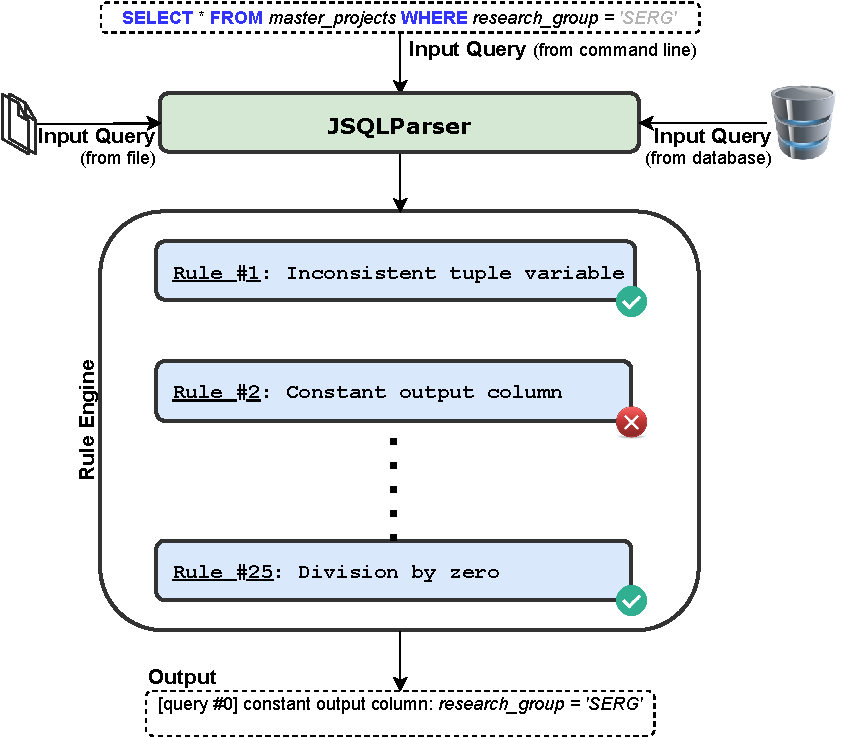
\includegraphics{img/tool_flow.pdf}
    \caption{Overall flow of the semantic bug detection tool}
    \label{fig:tool_flow}
\end{figure}

The detection strategies for each of the semantic bugs described in the previous sections are implemented as individual rules which make use of the visitor design pattern to parse SQL queries in search for different semantic bugs. Each rule focuses on detecting a single bug type. Furthermore, the tool is easily open for extension allowing for the implementation of numerous other rules for detecting other types of issues. Since for most rules there are a number of similarities such as parsing the queries in search for table sources or tuple variable names, there is a common interface shared by all the rules. 
One key aspect that we wanted to have for our tool was the ease of adding other rules in the future. In our current framework, this can easily be done by creating a new Java class and implementing the main interface which, among others, already takes care of parsing SQL queries. Developers then only have to override the methods for which custom functionality for the detection strategy is needed. This, for example, results in being able to write complicated heuristics for the rules without having to rewrite the parsing logic which saves both time as well as potential mistakes. Another important aspect is that rules can better be tested by only focusing on the new functionality which is specifically tailored for the detection strategy since the parsing logic is already tested by our framework.

The tool has three different modes of operation. In the first one, a query is entered via the command line and all the rules will be checked for finding semantic bugs in the input. This can be used whenever a fast check needs to be run for a single query in order to validate if this is semantically correct or not. The second mode of operation allows for an input file to be specified as input. The tool will then read all the queries from the file, which should be separated by a semicolon character (\sql{;}) and will display all the errors it detected for each of the SQL queries present in the file. This setting is perhaps more useful for conducting analysis on a larger input dataset. Finally, in the third mode of operation, the tool makes use of the Spring framework in order to connect to a MySQL database for retrieving input queries and running the rules on these. This mode was used during this research for analysing the large dataset of SQL queries collected from StackOverflow posts. The tool then also saves the results in this database which can later be used for further analysis.

Each rule is heavily covered by unit tests which try to account for general as well as more special edge cases. In total, there are more than 150 unit tests for the 25 rules implemented for our detection tool. Other tests include an automated script which uses a collection of more than 500 manually verified queries that runs against the tool and compares the outcome to the expected result. Some other 50 queries were manually checked in order to verify they do not contain any semantic errors after which they were presented as input to the tool in order to verify no warnings are raised, and later were added to the automated tests as well. The overall code quality for the tool was tracked on Better Code Hub, achieving an overall score of 9 out of 10 for quality, with the only area where maximum points were not scored being the separation of concerns in modules due to the shared interface used by all our rules. The source code for the tool together with all other scripts used for testing and analysing the results for this project can be found in GitHub at the following link: \url{https://github.com/cldme/SQLBugFinder}.


\section{Validation}
\label{section:validation}

Apart from the various unit tests implemented for checking each rule, the tool was validated using a manual process of investigating more than 500 SQL queries and verifying whether the output of the tool was correct or not. For each of the 25 semantic bug detection rules implemented in our tool, a random set of 20 queries collected from StackOverflow posts, for which the tool reported semantic bugs, was first selected in order to be manually analysed. The tool was configured such that each rule was run in isolation, meaning that every rule was analysed in detail, separately from the others, in order to confirm the correctness of both the implementation as well as the underlying heuristics used. Whenever a semantic bug was erroneously reported by the tool for a specific query, the code was analysed and fixed.

Furthermore, the unit tests were also improved to ensure the issues would not appear at a later stage when further modifications might be made to the rule. If multiple issues were found for a specific rule, after the initial set of 20 queries was verified, the process was restarted by selecting a new random set of 20 queries from the dataset for which the tool reported semantic bugs for the rule that was being checked. When no more errors were detected in the random sample, or none of the reported errors could be addressed, due to the fact that the query could not be parsed properly by the JSQLParser library or otherwise, the rule was considered to be sufficiently checked.
A dataset of roughly 500 queries was created, where for each rule the final set of 20 randomly selected queries together with the semantic bugs reported by the tool are registered. Furthermore, a script was implemented which uses this dataset together with the expected output to perform automated tests on the tool, in order to improve the testing of the rules.
